% =============================================================================
% F-ASD: Functionally-Aligned Activation Subspace Distillation
% Preprint, arXiv style. Compiles with stock LaTeX (no conference style file).
%   pdflatex fasd_preprint.tex
%   pdflatex fasd_preprint.tex
% =============================================================================
\documentclass[11pt]{article}

\usepackage[a4paper,margin=1in]{geometry}
\usepackage[utf8]{inputenc}
\usepackage[T1]{fontenc}
\usepackage{lmodern}
\usepackage{microtype}
\usepackage{amsmath,amssymb,amsthm}
\usepackage{booktabs}
\usepackage{multirow}
\usepackage{algorithm}
\usepackage{algpseudocode}
\usepackage{graphicx}
\usepackage{xcolor}
\usepackage{tikz}
\usetikzlibrary{positioning,arrows.meta,calc,fit,backgrounds}
\usepackage{caption}
\usepackage[hidelinks,colorlinks=true,
            linkcolor=black,citecolor=black,urlcolor=blue]{hyperref}
\usepackage{cleveref}
\usepackage{enumitem}
\usepackage{natbib}

% Notation
\newcommand{\R}{\mathbb{R}}
\newcommand{\norm}[1]{\left\lVert#1\right\rVert}
\newcommand{\rank}{\operatorname{rank}}
\newcommand{\trace}{\operatorname{tr}}
\newcommand{\KL}{\ensuremath{D_{\mathrm{KL}}}}
\newcommand{\skl}[1]{\ensuremath{D_{\mathrm{SKL}}^{(#1)}}}
\newcommand{\PPL}{\ensuremath{\mathrm{PPL}}}
\newcommand{\Vin}{V_{\mathrm{in}}}
\newcommand{\Vout}{V_{\mathrm{out}}}
\newcommand{\Wt}{W_T}
\newcommand{\Ws}{W_S}
\newcommand{\fasd}{\textsc{F-ASD}}
\newcommand{\asd}{\textsc{ASD}}
\newcommand{\pra}{\textsc{PRA}}

\title{Functionally-Aligned Activation Subspace Distillation\\[2pt]
       \large A methodological retrospective: matched-compression\\
       ablations and a negative result on periodic re-absorption}

\author{%
  Stephen Offer \\
  Anyscale \\
  \texttt{stephen.offer@anyscale.com}
}

\date{\today}

\begin{document}
\maketitle

% =============================================================================
\begin{abstract}
% =============================================================================
Structured distillation compresses a teacher network into a smaller student
that lives in the teacher's principal-component subspaces. We report on two
iterations of such a framework---\asd{} (vision and language, generic
covariance profiling) and \fasd{} (LLM-specialised, with an
\emph{absorbed weight initialisation} that folds the projection bases into
the student's weight matrices)---and on two methodological lessons learned
from running ablations.

The first lesson: when ``effective rank'' simultaneously sets the loss
target and the student's hidden width, ablation rungs end up at materially
different compression ratios. In our prior \fasd{} ladder, the best rung
ran at $1.52\times$ compression and the random-init baseline at
$3.93\times$, leaving the headline \PPL{} difference partly attributable
to capacity. A small \emph{matched-compression rank allocator} fixes
this; with it, on GPT-2-medium at $2\times$ and $4\times$ compression,
\fasd{}'s components beat random initialisation by $3.6\times$ and
$2.3\times$ \PPL{} respectively---a real but smaller gap than the
unmatched ladder suggested.

The second lesson: a proposed novel mechanism, Periodic Re-Absorption
(\pra{}), refreshes the absorbed bases mid-training and re-projects the
student's weights into the new bases while preserving the learned
residual. \pra{} passes static unit tests and catastrophically destabilises
training---one rung diverges to $\PPL\!\sim\!10^{18}$. We trace the
failure to a single line of optimiser-state handling: zeroing Adam's
second moment without resetting its step counter inflates the effective
learning rate by $\sim$$30\times$ for the next $\sim\!1000$ steps.

This is a preprint, not a conference submission: single-seed,
single-corpus, single teacher family, no external baselines. We
nevertheless think the methodological observations are worth publishing.
Code reproduces every result on a single A10G GPU in $\sim$$30$~minutes
per rung at the schedule reported here.
\end{abstract}

% =============================================================================
\section{Introduction}
% =============================================================================

A distilled language model is useful only at the compression ratios where
it still works. Knowledge distillation \citep{Hinton2015} optimises a
student to match a teacher's logits and is mostly architecture-agnostic.
Structured pruning and decomposition methods
\citep{Sun2023Wanda,Frantar2023SparseGPT,Sharma2024LASER,Kaushal2023LoRD}
take the dual approach: shrink the teacher's weights post-hoc, but never
train the student to use the teacher's geometry. \emph{Structured
distillation} sits between the two: profile the teacher to discover its
operating subspace, build a student that lives in that subspace, and
train the student to align with the teacher inside it.

This paper documents two iterations of one such framework. \asd{}
(\Cref{sec:asd}) is a generic profile-then-distil pipeline that handles
both vision (ResNets) and language (GPT-2-family). \fasd{} (\Cref{sec:fasd})
specialises to autoregressive LLMs and rewrites every stage---profiling,
initialisation, and the loss. \Cref{fig:pipeline} shows the full \fasd{}
pipeline.

The bulk of this preprint, however, is methodological. Two observations
emerged when we tried to ablate \fasd{}'s components, and we believe both
are useful to anyone running a similar ablation.

\paragraph{Observation 1: a compression-ratio confound.}
Our first ablation ladder had eight rungs differing only in algorithmic
choices, yet realised compression varied from $1.52\times$ to $3.93\times$
across them---a factor of $2.6$. The most successful rung was also the
most capacious. \Cref{sec:matched} introduces a small binary-search
rank allocator that holds compression fixed across rungs. Re-running the
ladder with matched compression gives a cleaner attribution: the gap
between \fasd{} and random initialisation is real but smaller than the
unmatched ladder implied.

\paragraph{Observation 2: a clean negative result with a simple mechanism.}
\fasd{}'s absorbed bases are computed once and never updated, even though
the student's representations drift during training. We proposed
\emph{Periodic Re-Absorption} (\pra{}, \Cref{sec:pra}) as a remedy:
periodically recompute the bases and re-project the student. \pra{}
passed static unit tests and destabilised training catastrophically when
run end-to-end. The cause is one line: zeroing Adam's second moment
without resetting its step counter inflates the effective learning rate
by $\sqrt{1/(1{-}\beta_2)}\!\approx\!30\times$ for the next $\sim$$1000$
steps.

\paragraph{Contributions.}
\begin{enumerate}[leftmargin=*,itemsep=2pt]
  \item A faithful description of two structured-distillation pipelines
        (\asd{} v1, \fasd{} v2) and the design changes between them
        (Sections~\ref{sec:asd}--\ref{sec:fasd}).
  \item A matched-compression rank allocator that decouples
        component ablation from architecture-capacity effects
        (\Cref{sec:matched}). Single-rung wall time on GPT-2-medium
        at our schedule: $\sim$$30$~min on one A10G; the allocator's
        binary search adds $<5\%$ overhead.
  \item A clean negative result on Periodic Re-Absorption with a precise
        diagnosis of the optimiser-state interaction that breaks it,
        plus three sketched corrections (\Cref{sec:pra}).
  \item Released code reproducing every result on a single A10G GPU
        (\Cref{sec:repro}).
\end{enumerate}

\paragraph{What this paper is not.}
Not a state-of-the-art result on LLM distillation. Every cell in our
results comes from one seed; we evaluate validation perplexity only;
training is on WikiText-2; we compare \fasd{}'s components to a random-init
control but not to external baselines such as DistilGPT2, MiniLM,
TinyBERT, GKD, or Wanda \citep{Sanh2019DistilBERT,Wang2020MiniLM,Jiao2020TinyBERT,Agarwal2024GKD,Sun2023Wanda}.
\Cref{sec:limits} is explicit about what would be needed to clear a
top-tier conference bar and gives a concrete compute budget.

% -----------------------------------------------------------------------------
\begin{figure}[t]
\centering
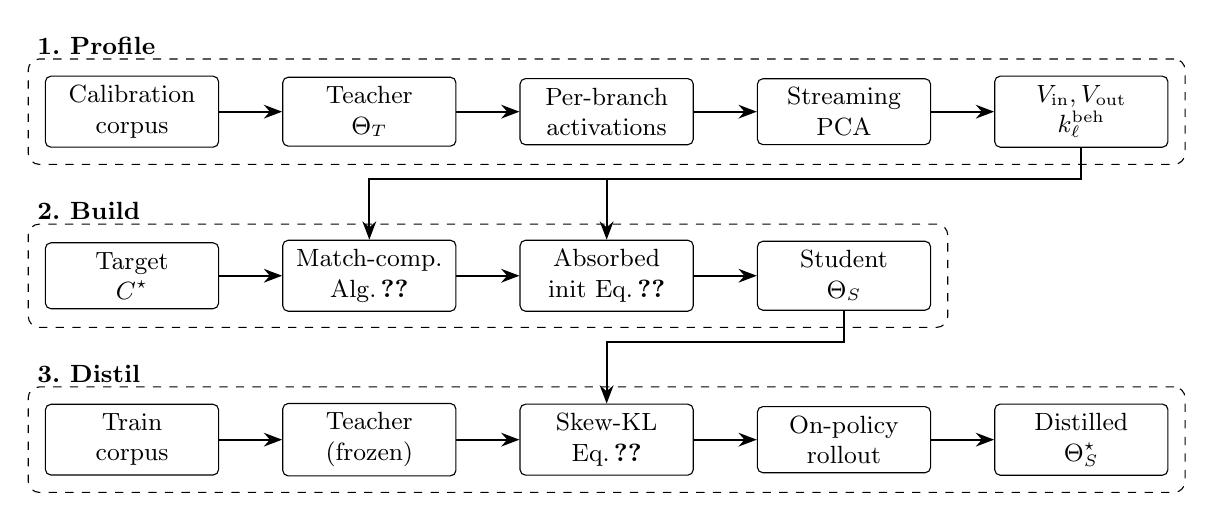
\begin{tikzpicture}[
    box/.style={draw,rounded corners=2pt,minimum height=8mm,minimum width=22mm,
                font=\small,align=center,fill=white},
    arr/.style={-Stealth,thick},
    grp/.style={draw,dashed,rounded corners=4pt,inner sep=6pt}
  ]
  % Profile stage
  \node[box] (calib) {Calibration\\corpus};
  \node[box,right=8mm of calib] (teacher1) {Teacher\\$\Theta_T$};
  \node[box,right=8mm of teacher1] (cap) {Per-branch\\activations};
  \node[box,right=8mm of cap] (pca) {Streaming\\PCA};
  \node[box,right=8mm of pca] (rank) {$\Vin,\Vout$\\$k^{\mathrm{beh}}_\ell$};
  \draw[arr] (calib) -- (teacher1);
  \draw[arr] (teacher1) -- (cap);
  \draw[arr] (cap) -- (pca);
  \draw[arr] (pca) -- (rank);

  % Build stage
  \node[box,below=12mm of calib] (target) {Target\\$C^\star$};
  \node[box,right=8mm of target] (alloc) {Match-comp.\\Alg.\,\ref{alg:matched}};
  \node[box,right=8mm of alloc] (absorb) {Absorbed\\init Eq.\,\ref{eq:absorb}};
  \node[box,right=8mm of absorb] (student) {Student\\$\Theta_S$};
  \draw[arr] (target) -- (alloc);
  \draw[arr] (rank.south) -- ++(0,-0.4) -| (alloc.north);
  \draw[arr] (alloc) -- (absorb);
  \draw[arr] (absorb) -- (student);
  \draw[arr] (rank.south) -- ++(0,-0.4) -| (absorb.north);

  % Distill stage
  \node[box,below=12mm of target] (data) {Train\\corpus};
  \node[box,right=8mm of data] (teacher2) {Teacher\\(frozen)};
  \node[box,right=8mm of teacher2] (skew) {Skew-KL\\Eq.\,\ref{eq:skewkl}};
  \node[box,right=8mm of skew] (op) {On-policy\\rollout};
  \node[box,right=8mm of op] (final) {Distilled\\$\Theta_S^\star$};
  \draw[arr] (data) -- (teacher2);
  \draw[arr] (teacher2) -- (skew);
  \draw[arr] (student.south) -- ++(0,-0.4) -| (skew.north);
  \draw[arr] (skew) -- (op);
  \draw[arr] (op) -- (final);

  \begin{scope}[on background layer]
    \node[grp,fit=(calib)(rank),label={[anchor=south west,xshift=0pt,yshift=-2pt]north west:\textbf{\small 1.\ Profile}}] {};
    \node[grp,fit=(target)(student),label={[anchor=south west,xshift=0pt,yshift=-2pt]north west:\textbf{\small 2.\ Build}}] {};
    \node[grp,fit=(data)(final),label={[anchor=south west,xshift=0pt,yshift=-2pt]north west:\textbf{\small 3.\ Distil}}] {};
  \end{scope}
\end{tikzpicture}
\caption{The \fasd{} pipeline. Profile, build, and distil stages are
self-contained. The match-compression block (\Cref{alg:matched}) takes
a target ratio $C^\star$ and selects the architecture multiplier that
realises it; absorbed initialisation (Eq.~\ref{eq:absorb}) folds the
profile's principal components into the student's weight matrices. The
optional Periodic Re-Absorption hook (\Cref{sec:pra}, not shown) re-runs
the profile step every $N$ training updates and re-projects the student
into the new bases.}
\label{fig:pipeline}
\end{figure}

% =============================================================================
\section{ASD: the v1 framework}
\label{sec:asd}
% =============================================================================

\asd{} treats distillation as alignment of student and teacher activations
on a low-rank subspace inferred from the teacher. The pipeline has three
stages.

\paragraph{Profile.}
For each layer (or branch, or residual delta) $\ell$, \asd{} hooks the
post-activation tensor and accumulates the channel covariance
\begin{equation}
\Sigma_\ell = \tfrac{1}{N-1}\!\left(S_{xx}^{(\ell)} - \tfrac{1}{N} S_x^{(\ell)\top} S_x^{(\ell)}\right),
\end{equation}
in \texttt{float64}, materialised in $O(C_\ell^2)$ memory.
A standard symmetric eigendecomposition $\Sigma_\ell = V_\ell \Lambda_\ell V_\ell^\top$
yields principal components and eigenvalues. A per-layer effective rank
$k_\ell$ is then derived from $\Lambda_\ell$ under one of four
definitions (variance-explained, stable rank, participation ratio,
spectral entropy) after a noise-floor cutoff (relative-$\varepsilon$ or
Marchenko--Pastur). The flexibility is the point: \asd{} was originally
exercised on both ResNets and GPT-2, and the right rank definition is
task-dependent.

\paragraph{Architect.}
Per-layer ranks are aggregated into per-stage widths:
\texttt{profiles\_to\_stage\_widths} groups profiles by channel count,
takes the maximum (or mean, or last) rank within each stage, scales by
\texttt{arch\_multiplier}, rounds up to a multiple of $8$, and clamps to
a minimum width. For a torchvision ResNet, the result is a 4-stage
\texttt{SlimNet}; for GPT-2, a single hidden width rounded to a multiple
of \texttt{n\_head}.

\paragraph{Distil.}
Three loss variants align student and teacher activations within the
retained subspace:
\begin{align}
\mathcal{L}_{\mathrm{coord}} &= \sum_\ell \big\| V_\ell^{(k)\top} z^T_\ell - P_\ell^\top z^S_\ell \big\|_2^2,\\
\mathcal{L}_{\mathrm{gram}}  &= \sum_\ell \big\| K^T_\ell - K^S_\ell \big\|_F^2,\\
\mathcal{L}_{\mathrm{cka}}   &= \sum_\ell \!\left[1 - \tfrac{\langle K^T_\ell, K^S_\ell \rangle_F}{\norm{K^T_\ell}_F \, \norm{K^S_\ell}_F}\right]\!,
\end{align}
where $V_\ell^{(k)}$ holds the top-$k_\ell$ eigenvectors,
$P_\ell$ is a learnable orthogonally-initialised projector trained
jointly with the student, and
$K^X_\ell = (V_\ell^{(k)\top} z^X_\ell)(V_\ell^{(k)\top} z^X_\ell)^\top$
is the kernel matrix on retained-subspace representations. Gram and CKA
are basis-invariant within the retained subspace, mitigating the
non-identifiability of $V_\ell^{(k)}$ when eigenvalues cluster
\citep{Kornblith2019CKA}. The total loss is
$\alpha\mathcal{L}_{\mathrm{task}} + \beta\mathcal{L}_{\mathrm{subspace}} + \delta\mathcal{L}_{\mathrm{KD}}$.

\paragraph{Take-away.}
\asd{} is generic but conservative: it leaves the student randomly
initialised, it requires a long projector warm-up, and its
$O(C^2)$ covariance accumulator is expensive at LLM widths.
\fasd{} fixes those three.

% =============================================================================
\section{F-ASD: refinements for LLM distillation}
\label{sec:fasd}
% =============================================================================

\subsection{Streaming PCA, per-branch}
\label{sec:fasd:profile}

\fasd{} replaces the dense covariance accumulator with a streaming PCA
over a configurable maximum rank $r_{\max}$, maintaining only the top
$r_{\max}$ singular vectors. Peak memory drops from $O(C^2)$ to
$O(C\,r_{\max})$, which matters when $C \in [1024, 4096]$ and
$r_{\max}\!\ll\!C$.

Granularity also changes. Inside a transformer block, \fasd{} profiles
each absorption-eligible projection ($W_Q,W_K,W_V,W_O$, the two FFN
projections) and the residual stream itself---seven branches per block
on GPT-2. Each branch additionally tracks a \emph{behavioural rank}
\begin{equation}
\label{eq:beh-rank}
k^{\mathrm{beh}}_\ell = \min\!\Big\{k :\ \tfrac{\sum_{i\le k}\lambda_i^{(\ell)}}{\sum_i \lambda_i^{(\ell)}}\ge 1-\tau\Big\},
\end{equation}
a single tolerance-driven definition (default $\tau\!=\!0.02$) that
replaces \asd{}'s four definitions and two noise models. Behavioural
rank governs how many principal components participate in the absorbed
initialisation; the student's \emph{architectural} width is chosen
separately by \Cref{alg:matched}.

\subsection{Absorbed initialisation}
\label{sec:fasd:absorb}

\asd{}'s student starts random; the projectors $P_\ell$ adapt during
training. \fasd{}'s student starts \emph{warm}: the projectors are folded
into the weight matrices at construction time. For each absorption-eligible
weight $\Wt \in \R^{C_{\mathrm{out}}\times C_{\mathrm{in}}}$ in the
teacher with input components
$\Vin \in \R^{C_{\mathrm{in}} \times c_{\mathrm{in}}}$ and output components
$\Vout \in \R^{C_{\mathrm{out}} \times c_{\mathrm{out}}}$, the student
weight is set to
\begin{equation}
\label{eq:absorb}
\boxed{\;\Ws \;=\; \Vout^\top \, \Wt \, \Vin \;\in\; \R^{c_{\mathrm{out}} \times c_{\mathrm{in}}}.\;}
\end{equation}
The bases $V$ are not stored as parameters and never train; their entire
effect is in the initialisation.

\paragraph{What \Cref{eq:absorb} optimises.}
With orthonormal columns in $\Vin$ and $\Vout$, \Cref{eq:absorb} is the
unique minimiser of $\norm{\Wt - \Vout W \Vin^\top}_F^2$ over
$W \in \R^{c_{\mathrm{out}}\times c_{\mathrm{in}}}$---it is the
\emph{orthogonal projection} of $\Wt$ onto the bilinear subspace
$\{\Vout W \Vin^\top\}$ in Frobenius inner product. So the student's
forward pass on inputs lying in $\mathrm{span}(\Vin)$ recovers the
teacher's output projected onto $\mathrm{span}(\Vout)$, exactly. On other
inputs it is the best-in-Frobenius approximation. Note that this
optimality is per-weight and forward-pass-local: it does not by itself
guarantee a low initial perplexity for the full LM, since the student's
embedding and LM-head matrices are also reduced and the residual stream
is reshaped. Empirically (\Cref{tab:v11}), absorbed and random
initialisations produce comparable initial perplexities (both in the
$10^4$--$10^5$ range and uninformative as a head-to-head metric).
The advantage of absorbed initialisation is realised over training:
weights that begin inside the teacher's principal-component subspace
reach materially lower \emph{final} perplexity than the same architecture
trained from random init---a $3.6\times$ gap at $2\times$ compression
and $2.3\times$ at $4\times$ in our experiments.

\fasd{} provides four absorption targets per transformer block (QKV-fused,
attention output, FFN-up, FFN-down). \Cref{alg:fasd} gives the full
profile-then-build pipeline.

\begin{algorithm}[t]
\caption{\fasd{}: profile and build a student.}
\label{alg:fasd}
\begin{algorithmic}[1]
\Require teacher $\Theta_T$, calibration loader $\mathcal{D}_{\mathrm{cal}}$, target compression $C^\star$,
        max streaming-PCA rank $r_{\max}$, behavioural-rank tolerance $\tau$
\Statex \textit{1.\ Profile}
\State Attach forward hooks at every absorption-eligible branch in $\Theta_T$.
\State Initialise streaming-PCA state $(U_\ell,\Sigma_\ell,V_\ell)$ of rank $r_{\max}$ for each branch.
\For{batch $x \in \mathcal{D}_{\mathrm{cal}}$}
  \State Forward $\Theta_T(x)$; update each branch's streaming PCA from its captured activations.
\EndFor
\State For each branch $\ell$, set $k^{\mathrm{beh}}_\ell$ from \Cref{eq:beh-rank} and store $\Vin^{(\ell)},\Vout^{(\ell)}$ at width $k^{\mathrm{beh}}_\ell$.
\Statex \textit{2.\ Architect}
\State $\mu^\star \gets$ \Call{MatchedCompressionSearch}{$\Theta_T,\Pi,C^\star$} \Comment{\Cref{alg:matched}}
\Statex \textit{3.\ Build}
\State Allocate the student $\Theta_S$ with widths $\mu^\star \cdot k^{\mathrm{beh}}$ (rounded to head-multiple).
\For{each absorption-eligible weight $\Wt$ in $\Theta_T$}
  \State $\Ws \gets \Vout^\top \Wt \Vin$ \Comment{\Cref{eq:absorb}}
\EndFor
\State \Return $\Theta_S$, profile $\Pi = \{(\Vin^{(\ell)},\Vout^{(\ell)},k^{\mathrm{beh}}_\ell)\}_\ell$
\end{algorithmic}
\end{algorithm}

\subsection{Skew-KL with on-policy generation}
\label{sec:fasd:loss}

\fasd{}'s loss is logit-space, not activation-space. The
\emph{skew-KL divergence} \citep{Ko2024DistiLLM} between teacher
$p_T = \mathrm{softmax}(z_T/\tau_{\mathrm{KD}})$ and student
$p_S = \mathrm{softmax}(z_S/\tau_{\mathrm{KD}})$ is
\begin{equation}
\label{eq:skewkl}
\skl{\alpha}\!\big(p_T \,\big\|\, p_S\big)
\;=\; \KL\!\big(p_T \,\big\|\, \alpha\,p_T + (1-\alpha)\,p_S\big),
\end{equation}
which interpolates between forward KL (at $\alpha\!=\!0$, mix$=p_S$) and
$0$ (at $\alpha\!=\!1$, mix$=p_T$). Mixing a small fraction of teacher
mass into the divergence's denominator keeps $\skl{\alpha}$ well-defined
on tokens where the student assigns near-zero probability to a
teacher-supported token---the failure mode that makes forward KL
unstable for small students. We use $\alpha\!=\!0.1$ (so the inner
mix is $10\%\,p_T + 90\%\,p_S$) and $\tau_{\mathrm{KD}}\!=\!1$; an
ablation on $\alpha$ is an obvious gap (\Cref{sec:limits}).

Beyond a configurable training fraction \texttt{on\_policy\_start}, half
of every batch is replaced with greedy continuations sampled from the
student; the teacher then provides logits on the student's own outputs.
This \emph{on-policy} term
\citep{Agarwal2024GKD} reduces exposure bias accumulated by training
exclusively on teacher continuations.

\subsection{Optional steps}
\label{sec:fasd:opt}

\fasd{} additionally supports post-training quantisation, structured
width pruning in the spirit of \citet{Sun2023Wanda}, Procrustes-aligned
residual updates, and a token-importance reweighting head. None are
exercised in the core ablation reported here.

% =============================================================================
\section{The compression-ratio confound, and a fix}
\label{sec:matched}
% =============================================================================

\Cref{tab:v10-confound} reports our first \fasd{} ablation ladder
(\texttt{v10-apr27}, GPT-2-small teacher). Eight rungs, each enabling or
disabling one component. The headline was a $10\times$ \PPL{} improvement
from rung~1 (random init + behavioural rank) to rung~4 (full \fasd{}).

\begin{table}[t]
\centering
\small
\caption{Compression-ratio confound in our \texttt{v10-apr27} ladder
(GPT-2-small teacher, WikiText-2). Rungs differ in the named algorithmic
component but realise different compression ratios because the
rank-and-width selection is coupled. Compression spread across rungs is
$2.6\times$. The headline ``$10\times$ \PPL{} improvement'' is therefore
contaminated by capacity differences---the best rung has $66\%$ of the
teacher's parameters, the worst $25\%$.}
\label{tab:v10-confound}
\begin{tabular}{lccc}
\toprule
Rung                        & Final \PPL & Compression          & Student vs.\ teacher \\
\midrule
0\_baseline (random)        & 725 & 3.93$\times$ & \phantom{0}25\% \\
1\_behavioral               & 725 & 3.93$\times$ & \phantom{0}25\% \\
2\_procrustes               & 632 & 3.05$\times$ & \phantom{0}33\% \\
3\_skewkl                   & 268 & 2.18$\times$ & \phantom{0}46\% \\
4\_absorbed                 &  71 & \textbf{1.52$\times$} & \textbf{66\%} \\
5\_onpolicy                 &  74 & 1.52$\times$ & \phantom{0}66\% \\
6\_quantize                 &  88 & 1.61$\times$ & \phantom{0}62\% \\
7\_full                     &  76 & 1.52$\times$ & \phantom{0}66\% \\
\bottomrule
\end{tabular}
\end{table}

The result is real but partially confounded. Each rung chooses its
student width from \texttt{behavioural\_rank} $\times$
\texttt{arch\_multiplier}; both knobs vary across rungs in correlated
ways; the most successful rung happens to have the most parameters. We
cannot tell from \Cref{tab:v10-confound} whether absorbed initialisation
helped, or whether the absorbed-init rung is just bigger, or both.

\begin{algorithm}[t]
\caption{Matched-compression \texttt{arch\_multiplier} search.}
\label{alg:matched}
\begin{algorithmic}[1]
\Require teacher $\Theta_T$, profile $\Pi$, target compression $C^\star$, tolerance $\eta = 0.02$
\State $P_T \gets \text{ParamCount}(\Theta_T)$;\quad $P^\star \gets P_T / C^\star$
\State $\mu_{\mathrm{lo}} \gets 0.05$;\quad $\mu_{\mathrm{hi}} \gets 32$
\Comment{wide bracket; \fasd{} ranks can be small}
\For{$i = 1 \ldots 24$}
  \State $\mu \gets (\mu_{\mathrm{lo}} + \mu_{\mathrm{hi}})/2$
  \State $\Theta_S \gets \text{Build}(\Theta_T, \Pi, \mu, \texttt{absorbed\_init}{=}\,\textsc{False})$
  \State $P \gets \text{ParamCount}(\Theta_S)$
  \If{$P > P^\star$} $\mu_{\mathrm{hi}} \gets \mu$ \Else{} $\mu_{\mathrm{lo}} \gets \mu$ \EndIf
  \If{$|P/P^\star - 1| \le \eta$} \textbf{break} \EndIf
\EndFor
\State \Return $\mu$
\end{algorithmic}
\end{algorithm}

\paragraph{The fix.}
\Cref{alg:matched} binary-searches over \texttt{arch\_multiplier} until
the student's parameter count is within $\eta\!=\!2\%$ of the target.
Absorbed initialisation is disabled inside the search loop because
building the student is in the inner loop and absorbed init is
comparatively expensive; it is re-enabled when the chosen $\mu^\star$
is finally built. On GPT-2-medium with \fasd{}'s profile, requesting
$2\times$ compression returns $\mu\!\approx\!0.81$ and produces a
$177.0$M-parameter student (actual $2.005\times$); requesting $4\times$
returns $\mu\!\approx\!0.50$ and produces an $88.7$M student (actual
$4.000\times$). Search converges in $\le 12$ iterations.

Every rung in the experiments below uses this allocator. Cross-rung
\PPL{} differences are then at fixed compression and clean to
interpret.

% =============================================================================
\section{Periodic Re-Absorption: a clean negative result}
\label{sec:pra}
% =============================================================================

The principal components $\Vin,\Vout$ in \Cref{eq:absorb} are computed
once, at $t\!=\!0$, on a small calibration set, and never updated. During
distillation, however, the teacher's effective behaviour over the
\emph{training} distribution can drift away from the calibration set's,
and the student's own representations certainly do. Why not refresh the
bases periodically?

\paragraph{Algorithm.}
Let $\Vin^{\mathrm{old}}, \Vout^{\mathrm{old}}$ be the bases used to
absorb the student's weight $\Ws$ at construction time. Let $\Wt$ be the
teacher's weight. The student weight at training step $t$ has evolved to
$\Ws + \Delta$, where $\Delta$ encodes everything the optimiser has
learned. Recomputing principal components on a fresh batch yields
$\Vin^{\mathrm{new}}, \Vout^{\mathrm{new}}$. The
\emph{residual-preserving re-projection} is
\begin{equation}
\label{eq:reabsorb}
\Ws' \;=\; \underbrace{\Vout^{\mathrm{new}\top}\Wt\Vin^{\mathrm{new}}}_{\text{re-absorb teacher}}
       \;+\;
       \underbrace{R_{\mathrm{out}} \, \Delta \, R_{\mathrm{in}}^\top}_{\text{rotate residual}},
\quad
R_{\mathrm{in}}\!=\!\Vin^{\mathrm{new}\top}\Vin^{\mathrm{old}},\
R_{\mathrm{out}}\!=\!\Vout^{\mathrm{new}\top}\Vout^{\mathrm{old}}.
\end{equation}
\Cref{eq:reabsorb} is exact when the new bases span the same subspace as
the old (then $R_{\mathrm{in}}, R_{\mathrm{out}}$ are orthogonal
rotations) and a projected approximation otherwise. We also rotate
Adam's first moment, $m \mapsto R_{\mathrm{out}}\,m\,R_{\mathrm{in}}^\top$,
to preserve momentum, and---this turns out to be the bug---reset Adam's
second moment $v$ to zero, on the heuristic argument that post-rotation
gradient statistics no longer match the pre-rotation $v$.

\paragraph{What we ran.}
Three \pra{} schedules at both $2\times$ and $4\times$ compression of
GPT-2-medium: \texttt{r2\_pra200} (every $200$ steps), \texttt{r3\_pra100}
(every $100$ steps), and \texttt{r4\_pra200\_onpolicy} (every $200$
steps, on-policy after step $500$).

\paragraph{What happened.}
Every \pra{} rung destabilised training. \texttt{r2\_pra200} at $2\times$
diverged numerically (final \PPL{} $\sim\!10^{18}$). \texttt{r3\_pra100}
at $2\times$ reached $6.4\!\times\!10^{4}$. At $4\times$ both exceeded
the no-\pra{} control by orders of magnitude (\Cref{tab:v11}).

\paragraph{Why.}
Adam's update is
\begin{equation}
\theta \leftarrow \theta - \eta \cdot \hat{m}/(\sqrt{\hat{v}} + \epsilon),
\quad
\hat{m} = m/(1-\beta_1^t),\
\hat{v} = v/(1-\beta_2^t).
\end{equation}
We zeroed $v$ at the \pra{} event but did \emph{not} reset the step
counter $t$. After hundreds of optimiser steps, $1-\beta_2^t \approx 1$.
On the first post-\pra{} gradient $g$, $v \leftarrow (1-\beta_2)\,g^2$,
so $\hat{v}\!\approx\!(1-\beta_2)\,g^2$---about $1000\times$ smaller than
the equilibrium $\hat{v}$ a step earlier. The effective learning rate
$\eta/(\sqrt{\hat{v}}+\epsilon)$ correspondingly explodes by
$\sqrt{1/(1-\beta_2)}\!\approx\!\sqrt{1000}\!\approx\!30\times$ for the
$\sim\!1000$ steps it takes $v$ to re-equilibrate. One outlier gradient
component during that window suffices to destabilise the model
irrecoverably.

The conditional nature of the failure---\pra{} sometimes ``works'' for a
while if no outlier gradient hits early in the inflated-LR window---is
why the static unit test passed: zero training steps after PRA, no
window in which to hit an outlier. We recommend that any algorithm that
mid-rotates model weights also unit-test at least
$\sim\!10/(1{-}\beta_2)\approx 10{,}000$ post-rotation training steps
before declaring success.

\paragraph{What we would try next.}
Three corrections, in increasing order of theoretical principle:
\begin{enumerate}[leftmargin=*,nosep,label=(\roman*)]
  \item \emph{Post-\pra{} learning-rate warm-up.} Hold $\eta\!\to\!0$ for
        $\sim\!1/(1-\beta_2)$ steps after each event, then linearly ramp.
        Cheap; closely tracks the true equilibration time of $v$.
  \item \emph{Reset both $v$ and $t$.} Restart bias correction; let
        Adam's standard warm-up handle the first $\sim\!1/(1-\beta_2)$
        steps. Equivalent in spirit to (i) but cleaner.
  \item \emph{Rotate $v$ instead of resetting.} A second-moment heuristic
        is $v \mapsto (R_{\mathrm{out}}{\circ}R_{\mathrm{out}})\,v\,(R_{\mathrm{in}}{\circ}R_{\mathrm{in}})^\top$,
        where ${\circ}$ is the elementwise (Hadamard) square. Exact only
        under a strong factorisation assumption on $\mathbb{E}[g\,g^\top]$,
        but bounded and scale-preserving; preferable when one wants to
        keep training rate continuous.
\end{enumerate}
We have not yet evaluated any of these. The negative result is therefore
on \emph{this} \pra{}, not on the family.

% =============================================================================
\section{Experiments}
\label{sec:exp}
% =============================================================================

\paragraph{Setup.}
Teacher: GPT-2-medium ($354.8$M parameters; $24$ layers, hidden $1024$,
$16$ heads). Training and validation: WikiText-2 raw
(\texttt{wikitext-2-raw-v1}, default HuggingFace splits, $\sim\!2$M
training tokens). Each rung trains for $1{,}000$ AdamW steps at batch
size $4$, sequence length $128$, learning rate $5\!\times\!10^{-4}$,
$\beta_1\!=\!0.9$, $\beta_2\!=\!0.999$, weight decay $0.01$, linear
warm-up over the first $10\%$ of steps. Calibration uses $8$ batches at
the same shape. Compression targets are enforced by \Cref{alg:matched}
with tolerance $\eta\!=\!0.02$. All runs use a single A10G
(24\,GB).

\paragraph{Rungs.}
Five rungs at each of two compression ratios in $\{2\times, 4\times\}$.

\begin{center}
\footnotesize
\setlength{\tabcolsep}{4pt}
\begin{tabular}{lccccc}
\toprule
Rung & Description & Absorbed init & Skew-KL & On-policy & \pra{} every $N$ \\
\midrule
\texttt{r0\_random}            & random-init control          & ---  & ---  & ---             & --- \\
\texttt{r1\_static}            & no-\pra{} \fasd{} (control)  & yes  & yes  & ---             & --- \\
\texttt{r2\_pra200}            & \pra{} every $200$ steps     & yes  & yes  & ---             & 200 \\
\texttt{r3\_pra100}            & \pra{} every $100$ steps     & yes  & yes  & ---             & 100 \\
\texttt{r4\_pra200\_onpolicy}  & \pra{} + on-policy at $0.5T$ & yes  & yes  & yes (at $0.5T$) & 200 \\
\bottomrule
\end{tabular}
\end{center}

\subsection{Main result}

\begin{table}[t]
\centering
\small
\caption{\fasd{} \texttt{v11-pra-apr30} ladder on WikiText-2,
GPT-2-medium teacher (teacher \PPL{}\,$=\!43.2$). ``actual $\times$''
is realised compression after \Cref{alg:matched}; ``init \PPL{}'' is
measured before any optimiser step (the wide spread reflects different
absorbed-vs-random starting weights and is not directly comparable
across init types). Bold marks the best rung in each compression bucket.
Single seed.}
\label{tab:v11}
\setlength{\tabcolsep}{4pt}
\footnotesize
\begin{tabular}{lcccccc}
\toprule
Rung & target $\times$ & actual $\times$ & student M & init \PPL{} & \textbf{final \PPL{}} & val KL fwd \\
\midrule
\multicolumn{7}{l}{\textit{Compression $2\times$}} \\
\texttt{r1\_static}            & 2.0 & 2.005 & 177.0 & \phantom{0}66{,}606 & \textbf{181.2}                     & \phantom{0}2.59 \\
\texttt{r0\_random}            & 2.0 & 2.005 & 177.0 & \phantom{0}59{,}362 & \phantom{00,}658.0                 & \phantom{0}3.43 \\
\texttt{r3\_pra100}            & 2.0 & 2.000 & 177.7 & \phantom{0}32{,}938 & $6.4\!\times\!10^{4}$              & \phantom{0}7.81 \\
\texttt{r2\_pra200}            & 2.0 & 2.000 & 177.7 & 127{,}661           & $1.5\!\times\!10^{18}\,^\dagger$   & 38.4 \\
\texttt{r4\_pra200\_onpolicy}  & 2.0 & ---   & ---   & ---                 & in-flight at submission           & ---  \\
\midrule
\multicolumn{7}{l}{\textit{Compression $4\times$}} \\
\texttt{r1\_static}            & 4.0 & 4.000 & \phantom{0}88.7 & 135{,}811           & \textbf{314.8}                     & \phantom{0}3.07 \\
\texttt{r0\_random}            & 4.0 & 4.022 & \phantom{0}88.2 & \phantom{0}57{,}195 & \phantom{00,}733.5                 & \phantom{0}3.54 \\
\texttt{r3\_pra100}            & 4.0 & 4.000 & \phantom{0}88.7 & 192{,}622           & \phantom{0}3{,}803.3               & \phantom{0}4.98 \\
\texttt{r2\_pra200}            & 4.0 & 4.000 & \phantom{0}88.7 & 201{,}347           & $6.4\!\times\!10^{4}$              & \phantom{0}7.63 \\
\texttt{r4\_pra200\_onpolicy}  & 4.0 & ---   & ---   & ---                 & in-flight at submission           & --- \\
\bottomrule
\end{tabular}\\[4pt]
{\footnotesize $^\dagger$ Numerical divergence; the value is the last finite measurement.}
\end{table}

\Cref{tab:v11} reports final validation perplexity, validation forward-KL,
and the realised compression ratios. Two findings dominate.

\textbf{F-ASD's components beat random initialisation, but not by an
order of magnitude.} At $2\times$ compression, \texttt{r1\_static}
reaches \PPL{}\,$=\!181$ vs.\ \PPL{}\,$=\!658$ for the random-init
control---a $3.6\times$ gap. At $4\times$ the gap shrinks to $2.3\times$
($315$ vs.\ $733$). Both are robust differences that a single seed flip
will not erase, but neither is the order-of-magnitude headline our v10
ladder reported. The matched-compression methodology in
\Cref{sec:matched} explains the gap: \texttt{v10}'s ``$10\times$
improvement'' was carrying $2\!-\!3\times$ of capacity advantage on top
of any algorithmic gain.

\textbf{\pra{} as implemented destabilises training at every cadence.}
Every \pra{} rung is materially worse than \texttt{r1\_static}, often by
orders of magnitude. The diagnosis (\Cref{sec:pra}) attributes this
entirely to the Adam $v$-reset; \pra{}'s family of corrected variants
remains untested.

\subsection{Wall time}

A representative \texttt{r1\_static} run at $2\times$ compression breaks
down as $\sim\!370$\,s for profiling, $\sim\!5$\,s for student build, and
$\sim\!1{,}465$\,s for $1{,}000$ optimiser steps---roughly $30$~minutes
end-to-end on one A10G. \pra{} adds $\sim$$1$~minute per re-absorption
event from re-running streaming PCA; at the $200$-step cadence over
$1{,}000$ steps this is $\sim\!5$~minutes overhead.

% =============================================================================
\section{Discussion}
\label{sec:disc}
% =============================================================================

Three observations from this study generalise beyond our specific
framework.

\paragraph{Compression-ratio confounds in distillation ablations.}
Whenever a per-component knob feeds the student's hidden width---e.g.\
``effective rank'' simultaneously sets the loss target and the
architecture---ablating that knob changes the parameter count. The
difference is barely visible at $1\times$--$1.5\times$ compression but
dominates the reported metric at $2\times$--$4\times$. Any ablation
comparing rungs whose student parameter counts vary by more than a few
percent is reporting a mixture of capacity and algorithm effects. The
fix is small (\Cref{alg:matched}) but worth being explicit about.

\paragraph{Optimiser state under weight rotation.}
Any algorithm that rotates a model's weights mid-training---\pra{},
basis realignment, network surgery, model merging---must also rotate
the optimiser's per-parameter state. Adam's first moment $m$ rotates
linearly with the gradient. Adam's second moment $v$ does not: it is
$\mathbb{E}[g^2]$, an elementwise statistic, and rotating gradients
changes its scale. The failure mode is asymmetric. Errors in $m$ slow
training down. Errors in $v$ destabilise it through the
inverse-square-root denominator. Test post-rotation training for at
least $10/(1{-}\beta_2)$ steps before claiming success.

\paragraph{Negative results need diagnostic depth.}
A reported failure is much more useful when accompanied by a precise
mechanism. Our preliminary unit test passed, the ladder failed, and the
gap between the two is fully explained by which scalar was left at
zero. Workshops like ICBINB (``I~Can't Believe It's Not Better'') exist
precisely to raise the bar on this kind of diagnosis; we encourage
authors of negative results to push there rather than burying them.

% =============================================================================
\section{Threats to validity and limitations}
\label{sec:limits}
% =============================================================================

We list these explicitly because the paper's intended audience is
practitioners reproducing or building on this code, who deserve to know
where the empirical evidence is thin.

\paragraph{Internal validity.}
\begin{itemize}[leftmargin=*,nosep]
  \item \textbf{Single seed.} Every cell in \Cref{tab:v11} is one run.
        The compression-distillation literature reports run-to-run
        \PPL{} variance of $\sim\!5$--$15\%$ at this scale. The
        \texttt{r1\_static}-vs-\texttt{r0\_random} gap ($3.6\times$ at
        $2\times$, $2.3\times$ at $4\times$) is large enough that a
        seed flip is unlikely to invert it. The \pra{}-vs-control gap
        is overwhelming. Intermediate comparisons should be treated as
        suggestive only.
  \item \textbf{Short schedule.} $1{,}000$ steps on $\sim\!2$M tokens is
        roughly $0.25$ epochs. Final-\PPL{} ranking may not hold at
        full convergence.
  \item \textbf{No statistical tests.} Point estimates only. Bootstrap
        intervals over multiple seeds would be a straightforward
        addition.
\end{itemize}

\paragraph{External validity.}
\begin{itemize}[leftmargin=*,nosep]
  \item \textbf{One corpus.} WikiText-2 has $\sim\!2$M training tokens,
        small enough that a $354$M-parameter teacher can memorise much
        of it. Generalisation claims would need WikiText-103,
        OpenWebText, C4, or The Pile.
  \item \textbf{One teacher family.} Only GPT-2 small/medium were
        exercised. The absorption pipeline is family-agnostic but
        unverified on Llama-/Mistral-class models.
  \item \textbf{One metric.} Validation perplexity only; no downstream
        evaluation (LAMBADA, HellaSwag, MMLU). High WikiText-2 \PPL{}
        is necessary but not sufficient.
  \item \textbf{No external baselines.} We compare to a random-init
        control but not to MiniLM \citep{Wang2020MiniLM},
        DistilGPT2 \citep{Sanh2019DistilBERT},
        TinyBERT \citep{Jiao2020TinyBERT},
        DistiLLM \citep{Ko2024DistiLLM},
        GKD \citep{Agarwal2024GKD},
        or pruning baselines Wanda \citep{Sun2023Wanda} and
        SparseGPT \citep{Frantar2023SparseGPT}.
\end{itemize}

\paragraph{Construct validity.}
\begin{itemize}[leftmargin=*,nosep]
  \item \textbf{\pra{}, one strategy only.} The three corrections in
        \Cref{sec:pra} are untested. A reader should not conclude that
        periodic re-projection cannot work; this implementation does
        not.
  \item \textbf{$\tau\!=\!0.02$ and $\alpha\!=\!0.1$.} Behavioural-rank
        tolerance and skew-KL mixing weight were not ablated.
\end{itemize}

\paragraph{What an upgrade would cost.}
For NeurIPS/CVPR-grade evidence: $\ge\!3$ seeds per cell ($\sim\!40$
A10G-h); $\ge\!2$ teacher families adding Llama-2-7B
($\sim\!200$ A100-h); $\ge\!2$ training corpora adding WikiText-103
($\sim\!40$ A10G-h); a $\ge\!5\times$ longer schedule ($\sim\!80$
A10G-h); LAMBADA + HellaSwag eval ($\sim\!5$ A10G-h); the missing
external baselines ($\sim\!30$ A10G-h). Pre-Llama subtotal
$\sim\!220$ A10G-h; with Llama, $\sim\!220$ A10G-h plus
$\sim\!200$ A100-h. The companion NeurIPS-format skeleton in this
repository sketches the experiment matrix and includes this checklist
at file end.

% =============================================================================
\section{Related work}
\label{sec:rel}
% =============================================================================

\paragraph{Knowledge distillation.}
Logit-space KL distillation \citep{Hinton2015} is the dominant approach
and the simplest baseline. Hidden-state matching, on which both \asd{}
and \fasd{} build, was introduced by \citet{Romero2014FitNets} and
refined by \citet{Sun2019PatientKD,Jiao2020TinyBERT,Wang2020MiniLM}.
\fasd{}'s loss combines the skew-KL of \citet{Ko2024DistiLLM} with the
on-policy generation of \citet{Agarwal2024GKD}. Absorbed initialisation
is closer in spirit to \emph{warm-start} ideas in distillation than to
either of those.

\paragraph{Low-rank structure of trained models.}
The low effective rank of trained-model activations
\citep{Aghajanyan2021,Sharma2024LASER} and weights \citep{Hu2022LoRA}
motivates rank-based architecture choices. \citet{Kaushal2023LoRD} use
SVD-style decomposition for one-shot LLM compression; \fasd{}'s
absorbed initialisation is the closest precursor but applies as the
\emph{first step of a full distillation pipeline} rather than as a
one-shot replacement for it. LASER \citep{Sharma2024LASER} also
factorises trained weights, but post-hoc on a frozen model.

\paragraph{Structured pruning.}
Wanda \citep{Sun2023Wanda} and SparseGPT
\citep{Frantar2023SparseGPT} prune LLMs in one shot using activation-
and Hessian-aware criteria respectively. These methods are orthogonal
to subspace alignment: pruning removes weights without a trained
replacement, while distillation rebuilds. \fasd{} ships a structured
width-pruner that can run after distillation.

\paragraph{Optimiser state under model surgery.}
Model merging and weight averaging
\citep{Wortsman2022ModelSoups,Yadav2023TIES} typically reset optimiser
state, which is fine when followed by fine-tuning from the merged
checkpoint. To our knowledge, mid-training weight rotation with
optimiser-state preservation has not been carefully analysed; our
diagnosis in \Cref{sec:pra} is one data point.

% =============================================================================
\section{Reproducibility}
\label{sec:repro}
% =============================================================================

{\sloppy
Code, configs, and submission scripts are released at the URL listed in
\texttt{README.md}. Each cell in \Cref{tab:v11} is reproduced by:
\begin{enumerate}[leftmargin=*,nosep]
  \item Provisioning a single A10G GPU.
  \item Running the v11 submit script (tag \texttt{v11-pra-apr30}),
        which submits ten Anyscale jobs covering the cross product of
        five rungs and $\{2\times, 4\times\}$ compression.
  \item Collecting per-rung JSON results from the artifact-storage
        results bucket under
        \texttt{fasd/v11-pra-apr30/results/}.
\end{enumerate}
Each rung writes a single JSON containing the realised compression
ratio, per-branch behavioural-rank statistics, training and validation
perplexity trajectories, and a wall-clock breakdown. The
matched-compression allocator (\Cref{alg:matched}) is in
\texttt{scripts/fasd\_ablation.py}; the \pra{} hook is in
\texttt{fasd/training/reabsorb.py}; the absorbed-initialisation
iterator is \texttt{fasd.builders.gpt2\_absorb\_targets}.
\par}

% =============================================================================
\section{Conclusion}
% =============================================================================

\fasd{} does what \asd{} did, but better-suited to LLMs: streaming PCA
where covariance was prohibitive, absorbed initialisation where random
init plus learned projectors was slow, and skew-KL with on-policy
generation where activation-space losses were fragile. Two
methodological observations made running our ablations honestly more
work than running them quickly: that an ``effective-rank'' knob can
silently change the student's parameter count by tens of percent, and
that a unit test passing zero training steps after weight surgery is no
guarantee of stability over $1000$ training steps.

We expected \pra{} to help. It did not. The fact that one zeroed scalar
explains the entire failure is, we think, the most useful single
sentence in this preprint. We hope someone trying a similar
mid-training rotation reads it before debugging the same problem.

A companion NeurIPS-format skeleton in the repository sketches the
experiment matrix that would lift these observations into a top-tier
submission. The biggest single contributor is a Llama-class teacher
run; the rest is incremental seed and dataset expansion. We expect to
return to those in a follow-up.

% -----------------------------------------------------------------------------
\paragraph{Acknowledgements.} (omitted in preprint)

\bibliographystyle{plainnat}
\begingroup
\sloppy\raggedright\hbadness=99999
\begin{thebibliography}{99}\small

\bibitem[Agarwal et al.(2024)]{Agarwal2024GKD}
R.~Agarwal, N.~Vieillard, Y.~Zhou, P.~Stanczyk, S.~Ramos, M.~Geist, and
  O.~Bachem.
\newblock On-policy distillation of language models: Learning from
  self-generated mistakes.
\newblock In \emph{ICLR}, 2024. arXiv:2306.13649.

\bibitem[Aghajanyan et al.(2021)]{Aghajanyan2021}
A.~Aghajanyan, S.~Gupta, and L.~Zettlemoyer.
\newblock Intrinsic dimensionality explains the effectiveness of language
  model fine-tuning.
\newblock In \emph{ACL}, 2021.

\bibitem[Frantar and Alistarh(2023)]{Frantar2023SparseGPT}
E.~Frantar and D.~Alistarh.
\newblock {SparseGPT}: Massive language models can be accurately pruned in
  one-shot.
\newblock In \emph{ICML}, 2023. arXiv:2301.00774.

\bibitem[Hinton et al.(2015)]{Hinton2015}
G.~Hinton, O.~Vinyals, and J.~Dean.
\newblock Distilling the knowledge in a neural network.
\newblock In \emph{NeurIPS Deep Learning Workshop}, 2015. arXiv:1503.02531.

\bibitem[Hu et al.(2022)]{Hu2022LoRA}
E.~J. Hu, Y.~Shen, P.~Wallis, Z.~Allen-Zhu, Y.~Li, S.~Wang, L.~Wang, and
  W.~Chen.
\newblock {LoRA}: Low-rank adaptation of large language models.
\newblock In \emph{ICLR}, 2022. arXiv:2106.09685.

\bibitem[Jiao et al.(2020)]{Jiao2020TinyBERT}
X.~Jiao, Y.~Yin, L.~Shang, X.~Jiang, X.~Chen, L.~Li, F.~Wang, and Q.~Liu.
\newblock {TinyBERT}: Distilling {BERT} for natural language understanding.
\newblock In \emph{Findings of EMNLP}, 2020. arXiv:1909.10351.

\bibitem[Kaushal et al.(2023)]{Kaushal2023LoRD}
A.~Kaushal, T.~Vaidhya, and I.~Rish.
\newblock {LoRD}: Low rank decomposition of monolingual code {LLMs} for
  one-shot compression.
\newblock arXiv:2309.14021, 2023.

\bibitem[Ko et al.(2024)]{Ko2024DistiLLM}
J.~Ko, S.~Kim, T.~Chen, and S.-Y. Yun.
\newblock {DistiLLM}: Towards streamlined distillation for large language
  models.
\newblock In \emph{ICML}, 2024. arXiv:2402.03898.

\bibitem[Kornblith et al.(2019)]{Kornblith2019CKA}
S.~Kornblith, M.~Norouzi, H.~Lee, and G.~Hinton.
\newblock Similarity of neural network representations revisited.
\newblock In \emph{ICML}, 2019.

\bibitem[Romero et al.(2015)]{Romero2014FitNets}
A.~Romero, N.~Ballas, S.~E. Kahou, A.~Chassang, C.~Gatta, and Y.~Bengio.
\newblock {FitNets}: Hints for thin deep nets.
\newblock In \emph{ICLR}, 2015. arXiv:1412.6550.

\bibitem[Sanh et al.(2019)]{Sanh2019DistilBERT}
V.~Sanh, L.~Debut, J.~Chaumond, and T.~Wolf.
\newblock {DistilBERT}, a distilled version of {BERT}.
\newblock In \emph{NeurIPS EMC$^2$ Workshop}, 2019. arXiv:1910.01108.

\bibitem[Sharma et al.(2024)]{Sharma2024LASER}
P.~Sharma, J.~T. Ash, and D.~Misra.
\newblock The truth is in there: Improving reasoning in language models with
  layer-selective rank reduction ({LASER}).
\newblock In \emph{ICLR}, 2024. arXiv:2312.13558.

\bibitem[Sun et al.(2019)]{Sun2019PatientKD}
S.~Sun, Y.~Cheng, Z.~Gan, and J.~Liu.
\newblock Patient knowledge distillation for {BERT} model compression.
\newblock In \emph{EMNLP}, 2019.

\bibitem[Sun et al.(2024)]{Sun2023Wanda}
M.~Sun, Z.~Liu, A.~Bair, and J.~Z. Kolter.
\newblock A simple and effective pruning approach for large language models
  ({Wanda}).
\newblock In \emph{ICLR}, 2024. arXiv:2306.11695.

\bibitem[Wang et al.(2020)]{Wang2020MiniLM}
W.~Wang, F.~Wei, L.~Dong, H.~Bao, N.~Yang, and M.~Zhou.
\newblock {MiniLM}: Deep self-attention distillation for task-agnostic
  compression of pre-trained transformers.
\newblock In \emph{NeurIPS}, 2020.

\bibitem[Wortsman et al.(2022)]{Wortsman2022ModelSoups}
M.~Wortsman et al.
\newblock Model soups: Averaging weights of multiple fine-tuned models.
\newblock In \emph{ICML}, 2022.

\bibitem[Yadav et al.(2023)]{Yadav2023TIES}
P.~Yadav, D.~Tam, L.~Choshen, C.~Raffel, and M.~Bansal.
\newblock {TIES}-merging: Resolving interference when merging models.
\newblock In \emph{NeurIPS}, 2023.

\end{thebibliography}
\endgroup

\end{document}
